\chapter{Design}

With the requirements discussed in \autoref{sec:KubeLB}, the next step is to design the architecture and determine the technologies to be used.
Since the core product of Kubermatic is based on Kubernetes, the KubeLB project also has to be operated in this context.
To adapt concepts from KKP, the goal is to use a Kubernetes cluster for load balancing.
This promotes a homogeneous environment of Kubernetes clusters without introducing additional complexity of third party systems, which simplifies both the deployment and the maintenance of the KubeLB application.

\section{Manager}\label{sec:manager}

The Manager, as already explained in \autoref{sec:operator-pattern}, will serve as an operator and implement a controller comparable to \autoref{sec:controllers}.
Its task is to observe a CRD~(see \autoref{sec:custom-resource-definitions}) and operate the load balancers within the load balancer cluster.
Those CRDs hold the desired configuration for the load balancers and are called TCPLoadBalancer for Layer 4, and HTTPLoadBalancer for Layer 7 load balancing.
\\
Within the load balancer cluster, different Kubernetes resources are used to reflect this.
The deployment~(see \autoref{subsec:deployment}) creates the actual load balancer within the cluster.
The service~(see \autoref{subsec:service}) exposes the load balancer deployment to the outside via a service of type LoadBalancer.
It should be noted that the load balancer cluster requires a load balancer implementation.
This can be either a cloud provider, or an Open Source single cluster implementation.
\\
Since the created service is of type LoadBalancer, the status field of the service gets updated with the external IP address.
The Manager should observe this and set the status field within the CRD.
\\
For layer 7 implementation, the Manager makes use of the ingress~(see \autoref{subsec:ingress}), therefore an ingress controller~(see \autoref{sec:IngressController}) must be installed as well.

\section{Agent}\label{sec:agent}

The Agent runs inside a user cluster and watches for services and ingress resources.
If needed, it creates a CRD with the details needed for the Manager inside the load balancer cluster.
Since the Agent runs inside the user cluster, it can read the desired configurations of the service or ingress resource and create, modify or delete the CRD appropriately.
\\
Likewise, it is able to get the endpoints and open ports for a service, that are required for the load balancer.
Since the cluster size, i.e.\ the number of nodes, can change dynamically, it is also the Agent's task to update the changed endpoints of the user cluster for all CRDs within the load balancer cluster.
\\
In the case of layer 4 load balancing, the Agent also sets the IP address in the status field of the service, which is set inside the status field of the CRD by the Manger.
\\
To interact with the load balancer cluster, the Agent needs access to a namespace to deploy the CRDs inside.

\section{Layer 4}

\autoref{fig:kubelb-l4} illustrates the architecture of layer 4 load balancing.
Within the user cluster, the Agent observes the service resource.
If a user creates a service of type LoadBalancer, the Agent recognizes the service and creates a TCPLoadBalancer inside the load balancer cluster.
\\
The Manager observes the TCPLoadBalancer CRD, which contains the necessary information to configure the load balancer.
Based on this, the Manager creates or updates the load balancer deployment and the associated service.


\begin{figure}[H]
    \centering
    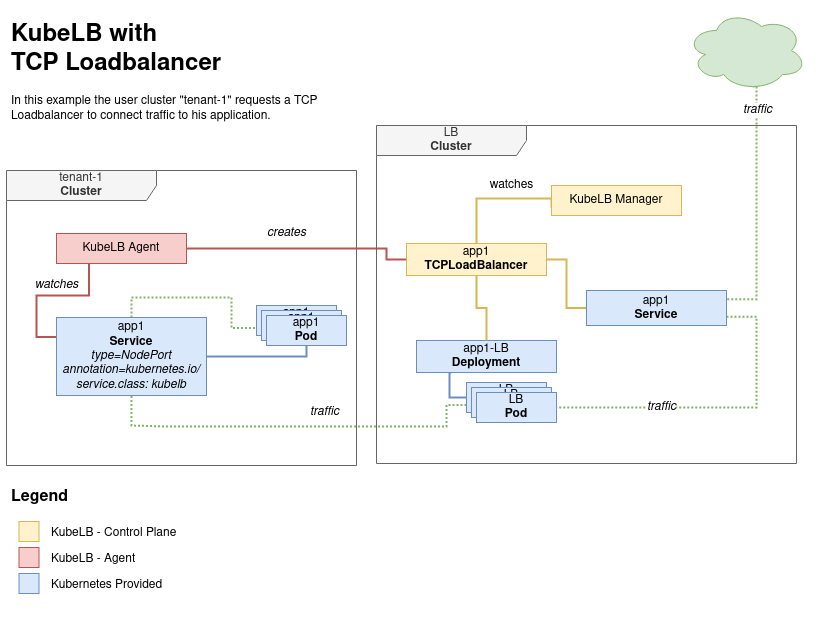
\includegraphics[width=1\linewidth]{media/06/kubelb-l4}
    \caption{"KubeLB Layer 4 architecture" by Kubermatic GmbH Apache License 2.0}
    \label{fig:kubelb-l4}
\end{figure}

\section{Layer 7}

Layer 7 load balancing introduces more complexity.
As \autoref{fig:kubelb-l7} shows, it relies on more components.
It is assumed that no ingress controller is installed inside the user cluster and KubeLB should fulfill the ingress, therefore some extra steps are required.
At first the service to expose via ingress could be of type ClusterIP, in this case it is not reachable for the load balancer inside the load balancer cluster.
In this case the Agent copies the existing service and creates a new one of type node port, so it is actually exposed and accessible to the load balancer.
\\
The second part is to create a TCPLoadBalancer, based on the copied service, inside the load balancer cluster.
Since KubeLB makes use of the ingress controller implementation, it needs some kind of connector to the user cluster.
Ingress is, by design, cluster based and only routable to internal services.
For that reason it is mandatory to have an internal load balancer service, accessible for the ingress controller.
It is not necessary to expose the load balancer, so the Agent sets the service type inside the TCPLoadBalancer to ClusterIP.
\\
At this point the Agent creates a HTTPLoadBalancer, based on the ingress inside the user cluster, inside the load balancer cluster.
The Manager takes care that the ingress is configured to use the corresponding load balancer service, which was created before.

\begin{figure}[H]
    \centering
    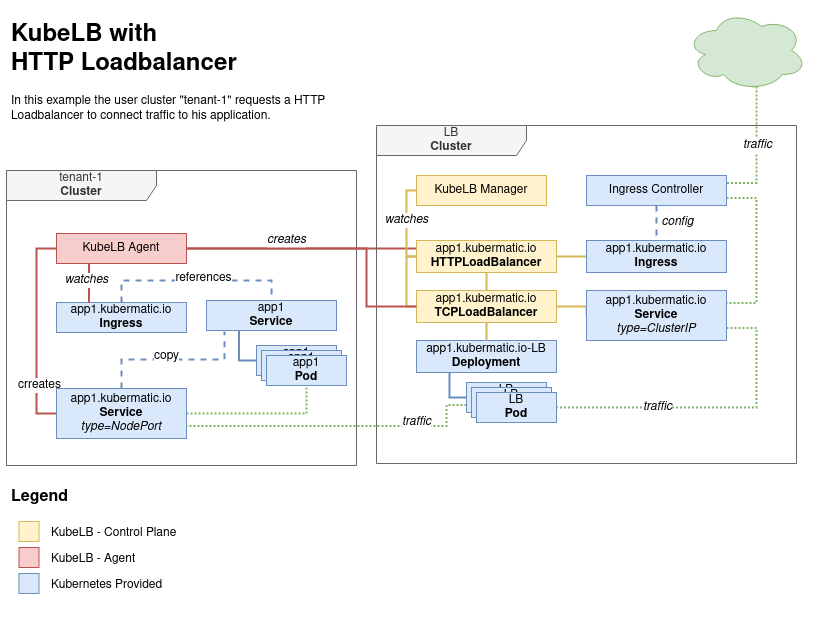
\includegraphics[width=1\linewidth]{media/06/kubelb-l7}
    \caption{"KubeLB Layer 7 architecture" by Kubermatic GmbH Apache License 2.0}
    \label{fig:kubelb-l7}
\end{figure}

\section{Envoy}\label{sec:envoy}

Envoy is chosen as a load balancer instance because of its design for large modern service oriented architectures and its high feature set.
Nginx and HA-Proxy offer similar functionalities, but are not initially developed for the required purposes inside a cloud native environment.
\\
The most important functions needed for KubeLB are summarized below:

\begin{itemize}
    \item \textit{L3/L4 filter architecture} \\
    The Envoy core is a L3/L4 network proxy, that is configurable via filter chains, allowing the proxy to perform different TCP/UDP tasks.
    \item \textit{HTTP L7 filter architecture} \\
    Since HTTP is widely used for applications to communicate, envoy offers an additional Layer 7 filter architecture on top, which can be used for various tasks like rate limiting, routing, forwarding and more.
    \item \textit{HTTP L7 routing} \\
    Envoy offers a special Layer 7 routing filter to make HTTP header based routing decisions and more.
    \item \textit{Advanced load balancing} \\
    It also implements a rich set of load balancing algorithms, as well as automatic retries, circuit breaking and more.
    \item \textit{Health checking} \\
    Envoy supports active and also passive health checking in order to determine healthy endpoint targets.
\end{itemize}

This is just a brief overview of the features of Envoy and what KubeLB is going to make use of.~\cite{WHAT-IS-ENVOY}
\\
Another important feature is Envoys data plane API.
In contrast to a control-plane the data-plane controls the data requests.
\\
To fulfill that purpose the Envoy API implements a data-plane.
In practice that means, that it is possible to control envoy proxies via this API.
This is very useful in cloud native environments, where services change their configuration on runtime, nodes get added or deleted and so on.
For that reason the Manager implements the envoy data-plane API and is in control of the configuration of all its load balancers.
